% 《泡泡知道自己在哪裡》童書排版
% 使用LaTeX創建專業童書排版

\documentclass[12pt,a4paper]{book}
\usepackage[utf8]{inputenc}
\usepackage{xeCJK}
\usepackage{fontspec}
\usepackage{graphicx}
\usepackage{tikz}
\usepackage{geometry}
\usepackage{xcolor}
\usepackage{tcolorbox}
\usepackage{setspace}
\usepackage{fancyhdr}

% 設置頁面
\geometry{
    paperwidth=20cm,
    paperheight=20cm,
    margin=1.5cm,
    showframe=false
}

% 設置中文字體
\setCJKmainfont{STSong}[
    BoldFont=STSong,
    ItalicFont=STKaiti
]

% 設置英文字體(圓潤的兒童字體)
\setmainfont{Comic Sans MS}[
    BoldFont=Comic Sans MS Bold
]

% 定義顏色
\definecolor{bubbleblue}{RGB}{227,242,253}
\definecolor{rainbowpink}{RGB}{255,192,203}
\definecolor{rainboworange}{RGB}{255,165,0}
\definecolor{rainbowyellow}{RGB}{255,255,0}
\definecolor{rainbowgreen}{RGB}{144,238,144}
\definecolor{rainbowpurple}{RGB}{221,160,221}
\definecolor{textblue}{RGB}{25,118,210}

% 定義泡泡樣式
\newcommand{\bubbletext}[1]{%
    \tikz[baseline=(char.base)]{%
        \node[draw,circle,minimum size=1.5em,fill=bubbleblue!30,text=textblue] (char) {#1};%
    }%
}

% 定義對話泡泡
\newcommand{\speechbubble}[1]{%
    \begin{tcolorbox}[
        colback=bubbleblue!20,
        colframe=textblue!50,
        boxrule=0.5pt,
        arc=3mm,
        left=1mm,
        right=1mm,
        top=1mm,
        bottom=1mm,
        fonttitle=\bfseries\large,
        title=\bubbletext{泡泡}
    ]
    #1
    \end{tcolorbox}%
}

% 定義音效文字
\newcommand{\soundeffect}[1]{%
    \textcolor{textblue}{\textbf{\Large #1}}%
}

% 定義頁面標題
\newcommand{\pagetitle}[1]{%
    \begin{center}%
    \textcolor{textblue}{\Huge\textbf{#1}}%
    \end{center}%
    \vspace{0.5cm}%
}

% 設置頁眉頁腳
\pagestyle{fancy}
\fancyhf{}
\renewcommand{\headrulewidth}{0pt}

% 開始文檔
\begin{document}

% 封面頁
\thispagestyle{empty}
\begin{center}
\vspace*{2cm}

% 封面插圖
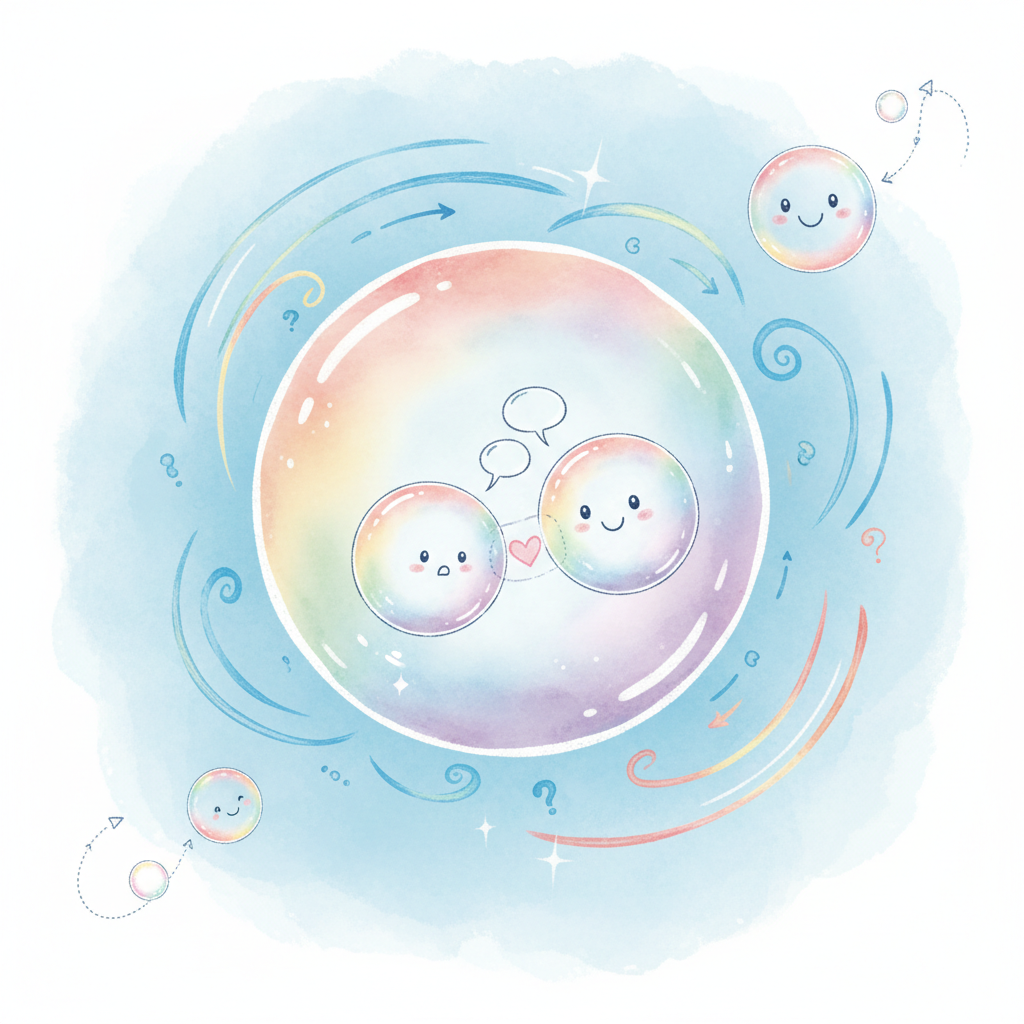
\includegraphics[width=12cm,height=12cm,keepaspectratio]{Cover.png}

\vspace{1cm}

% 書名
{\Huge\textcolor{textblue}{\textbf{泡泡知道自己在哪裡}}}

\vspace{0.5cm}

% 副標題
{\Large\textcolor{textblue}{寶寶的範疇思維書}}

\vspace{2cm}

% 作者信息
{\large\textcolor{textblue}{作者:[你的名字]}}

\vspace{1cm}

% 出版信息
{\small\textcolor{textblue}{2024年}}

\end{center}

% 第1頁:泡泡出生了
\newpage
\thispagestyle{empty}
\begin{center}

% 頁面插圖
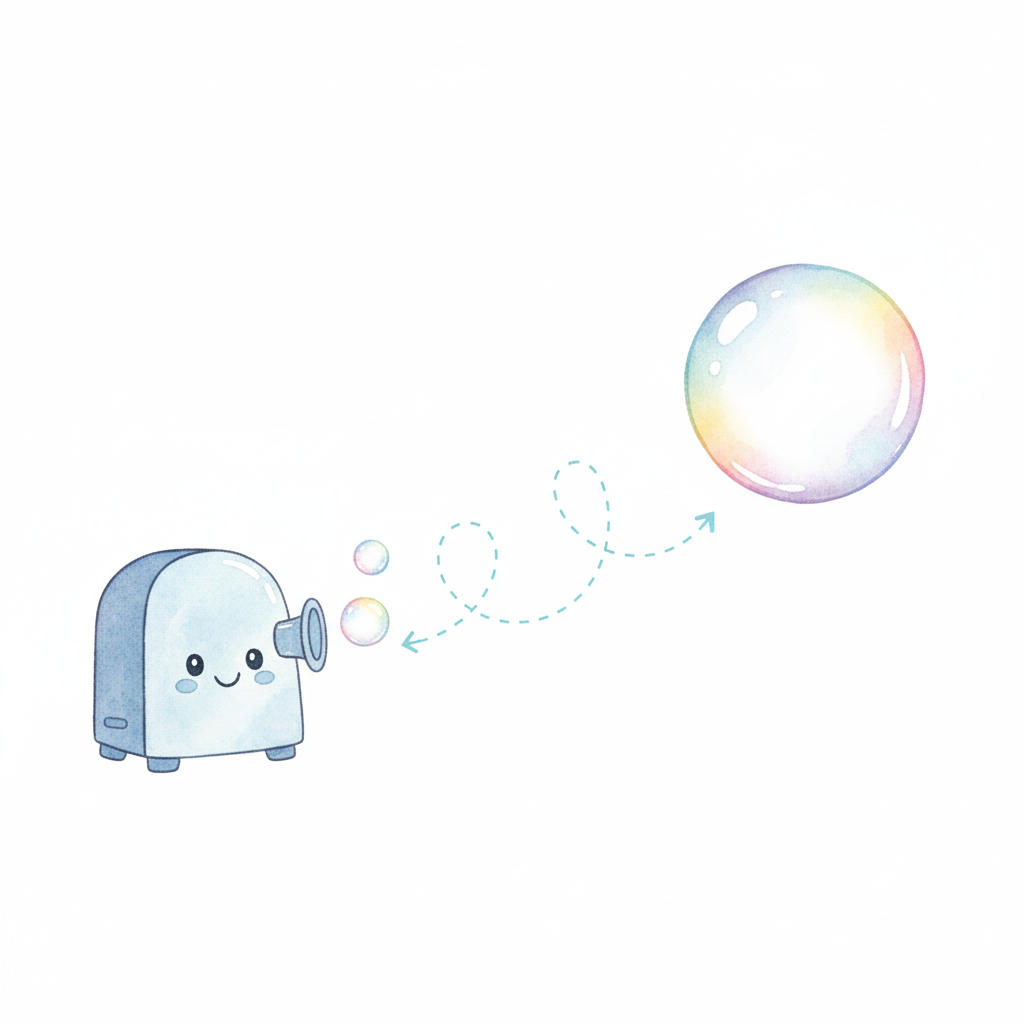
\includegraphics[width=15cm,height=15cm,keepaspectratio]{Page1.png}

\vspace{1cm}

% 文字內容
\soundeffect{噗噗噗...}

\vspace{0.3cm}

泡泡從泡泡機裡飛出來

\vspace{0.2cm}

圓圓的、透明的

\vspace{0.2cm}

\speechbubble{泡泡知道自己是泡泡}

\end{center}

% 第2頁:泡泡看到自己
\newpage
\thispagestyle{empty}
\begin{center}

% 頁面插圖
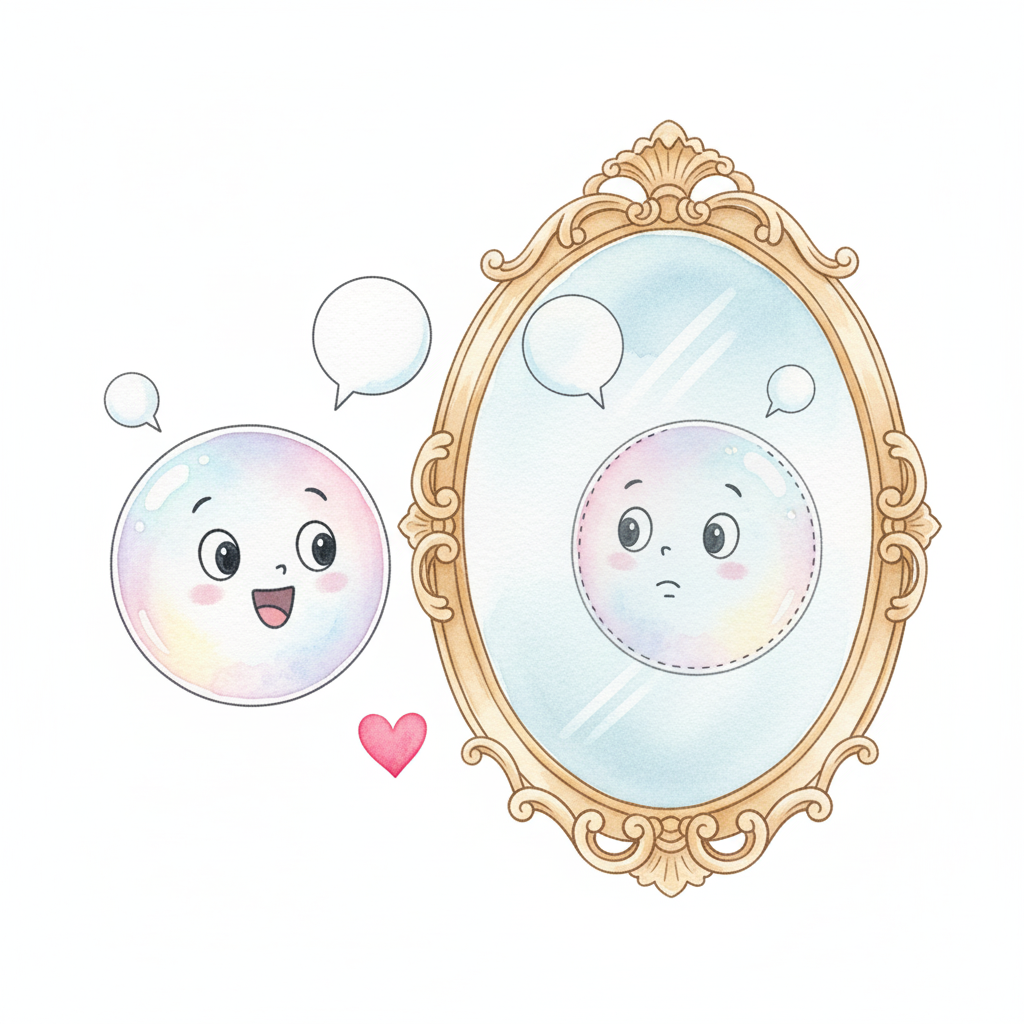
\includegraphics[width=15cm,height=15cm,keepaspectratio]{Page2.png}

\vspace{1cm}

泡泡在鏡子前

\vspace{0.2cm}

看到另一個泡泡

\vspace{0.3cm}

\speechbubble{那是誰?}

\vspace{0.2cm}

\speechbubble{是我!}

\end{center}

% 第3頁:泡泡的世界
\newpage
\thispagestyle{empty}
\begin{center}

% 頁面插圖

\includegraphics[width=15cm,height=15cm,keepaspectratio]{Page3.png}

\vspace{1cm}

泡泡裡有彩虹

\vspace{0.2cm}

泡泡外有風

\vspace{0.2cm}

泡泡知道:

\vspace{0.3cm}

\speechbubble{我在裡面,世界在外面}

\end{center}

% 第4頁:泡泡變大了
\newpage
\thispagestyle{empty}
\begin{center}

% 頁面插圖
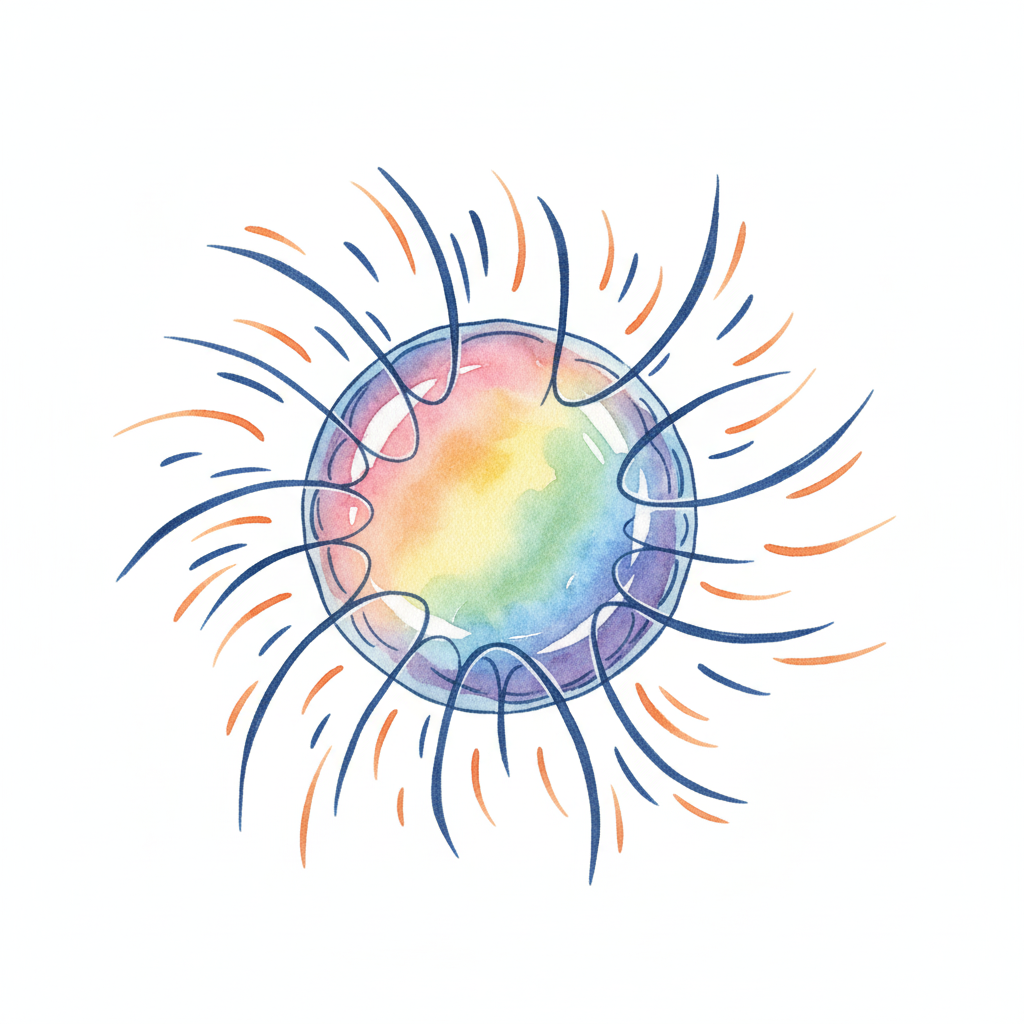
\includegraphics[width=15cm,height=15cm,keepaspectratio]{Page4.png}

\vspace{1cm}

\soundeffect{呼呼呼...}

\vspace{0.2cm}

泡泡越來越大

\vspace{0.2cm}

邊界越來越薄

\vspace{0.2cm}

快要...快要...

\end{center}

% 第5頁:泡泡破了
\newpage
\thispagestyle{empty}
\begin{center}

% 頁面插圖

\includegraphics[width=15cm,height=15cm,keepaspectratio]{Page5.png}

\vspace{1cm}

\soundeffect{啪!}

\vspace{0.2cm}

泡泡不見了

\vspace{0.2cm}

彩虹飛散了

\vspace{0.2cm}

風吹進來了

\end{center}

% 第6頁:新的泡泡
\newpage
\thispagestyle{empty}
\begin{center}

% 頁面插圖
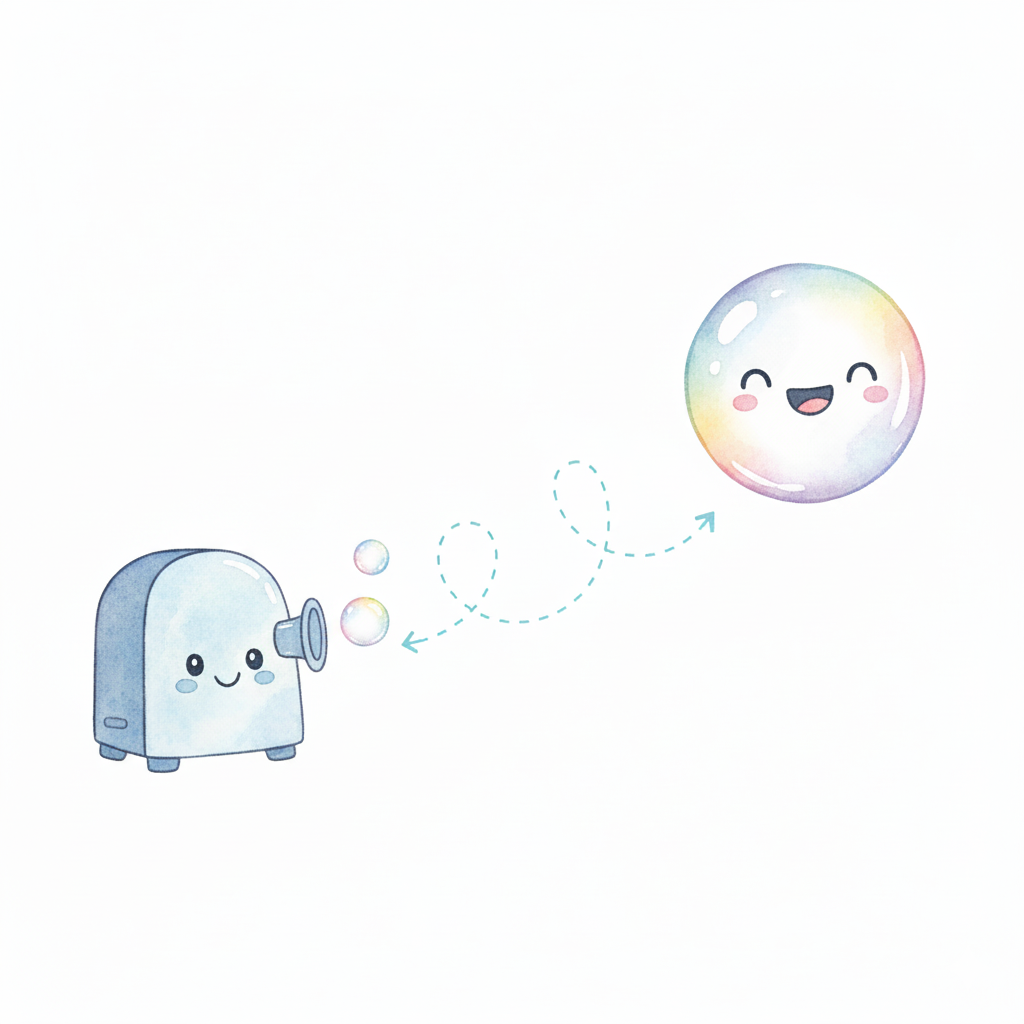
\includegraphics[width=15cm,height=15cm,keepaspectratio]{Page6.png}

\vspace{1cm}

\soundeffect{噗噗噗...}

\vspace{0.2cm}

又一個泡泡飛出來

\vspace{0.2cm}

圓圓的、透明的

\vspace{0.3cm}

\speechbubble{我又是泡泡了!}

\end{center}

% 第7頁:泡泡的朋友們
\newpage
\thispagestyle{empty}
\begin{center}

% 頁面插圖
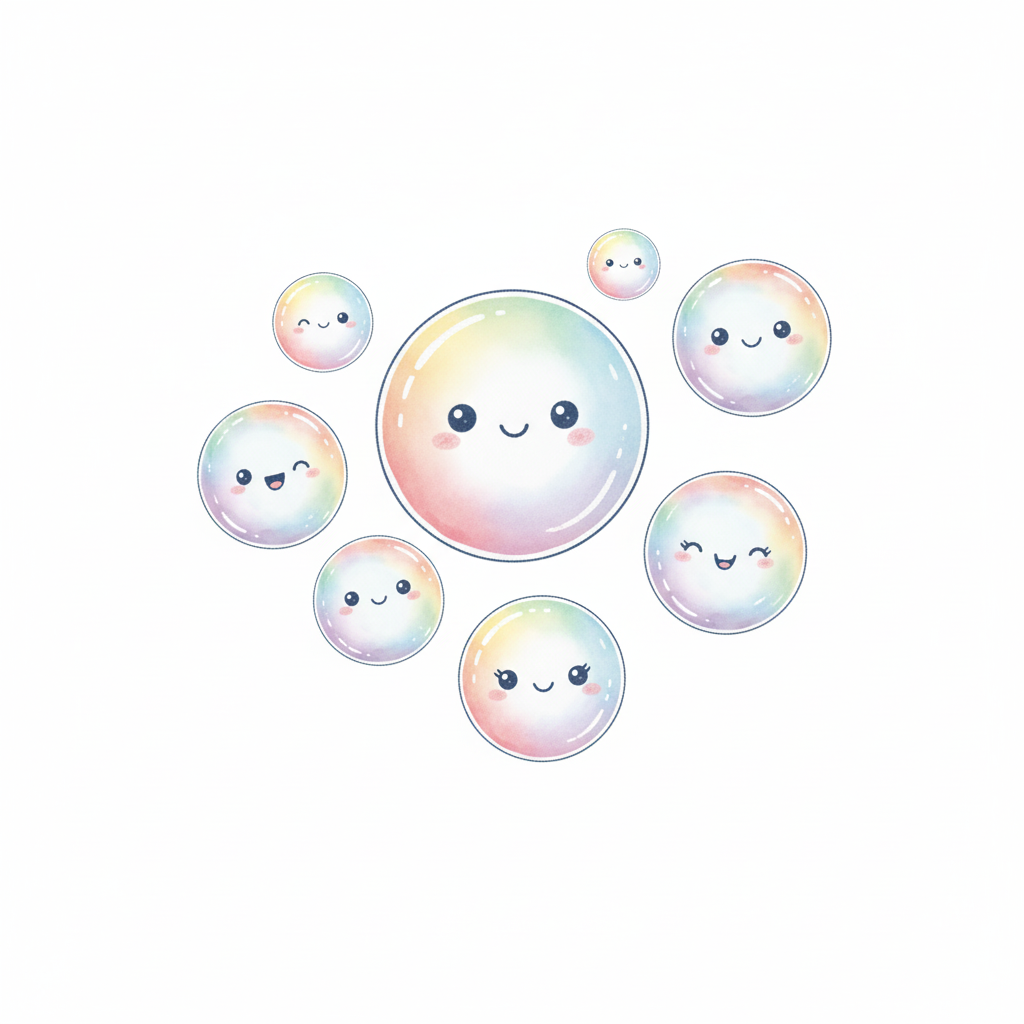
\includegraphics[width=15cm,height=15cm,keepaspectratio]{Page7.png}

\vspace{1cm}

好多泡泡!

\vspace{0.2cm}

每個泡泡都有自己的彩虹

\vspace{0.2cm}

每個泡泡都有自己的邊界

\vspace{0.2cm}

每個泡泡都知道自己在哪裡

\end{center}

% 第8頁:泡泡擁抱
\newpage
\thispagestyle{empty}
\begin{center}

% 頁面插圖
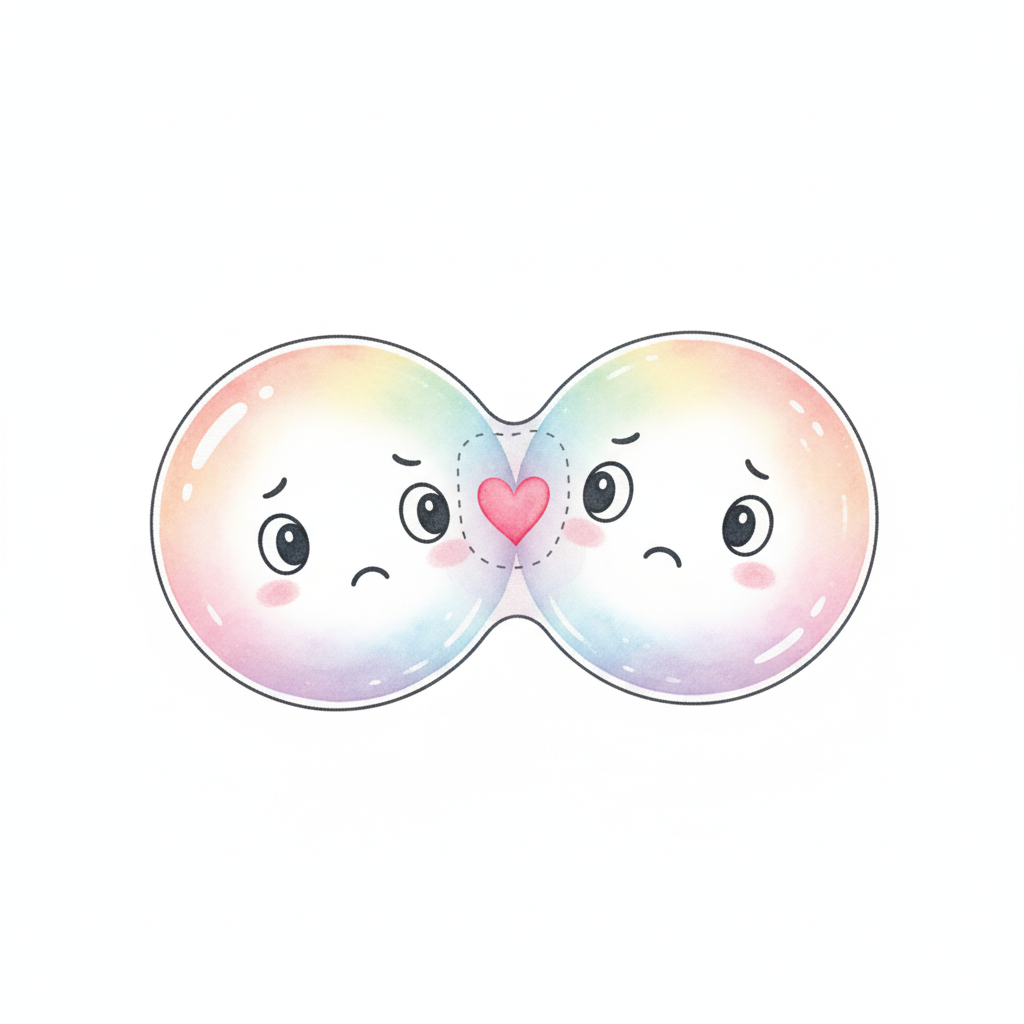
\includegraphics[width=15cm,height=15cm,keepaspectratio]{Page8.png}

\vspace{1cm}

兩個泡泡輕輕碰在一起

\vspace{0.2cm}

邊界變模糊了

\vspace{0.3cm}

\speechbubble{我們是一起的嗎?}

\vspace{0.2cm}

\speechbubble{我們還是分開的嗎?}

\end{center}

% 第9頁:泡泡融合
\newpage
\thispagestyle{empty}
\begin{center}

% 頁面插圖
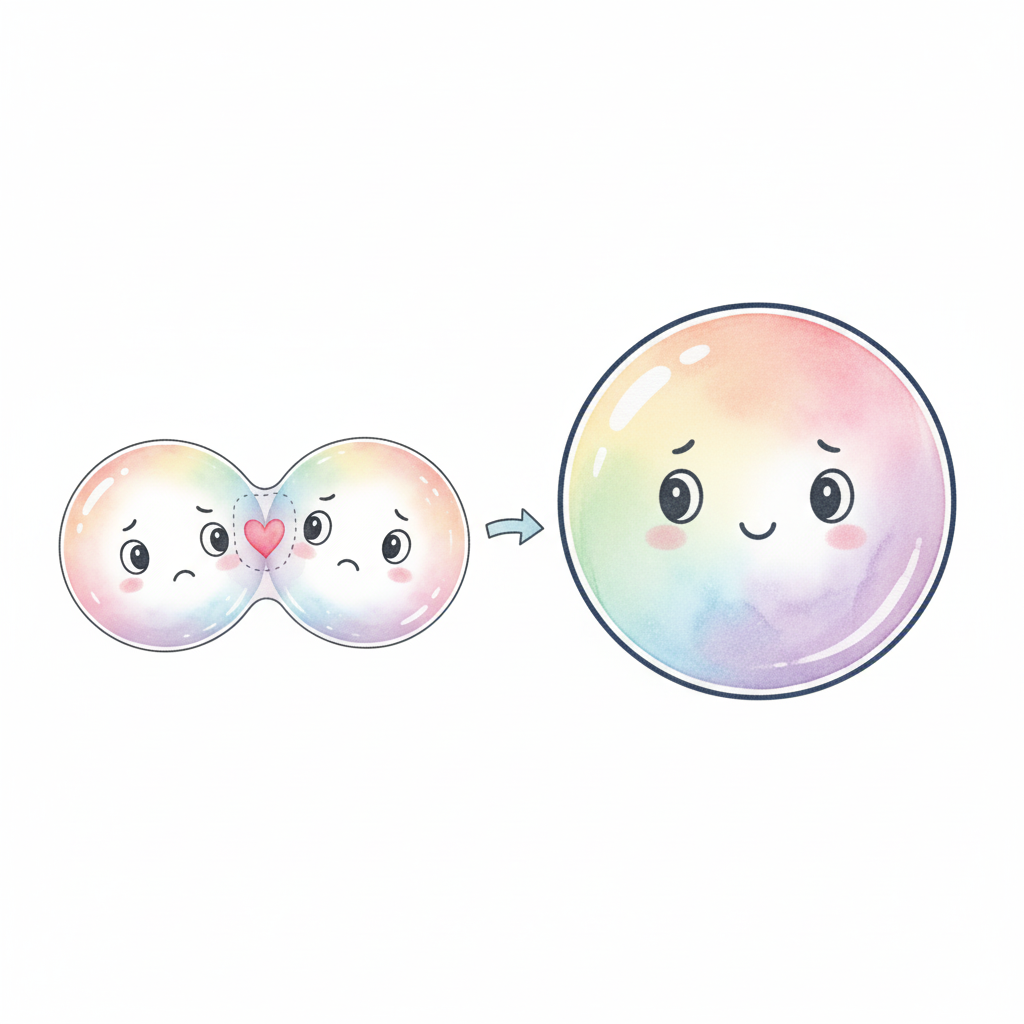
\includegraphics[width=15cm,height=15cm,keepaspectratio]{Page9.png}

\vspace{1cm}

變成一個大泡泡!

\vspace{0.2cm}

彩虹混合了

\vspace{0.2cm}

邊界重新畫了

\vspace{0.3cm}

\speechbubble{我們現在是一體的}

\end{center}

% 結束文檔
\end{document}
